\documentclass[UTF8]{ctexart}
\usepackage[a4paper,margin=1.8cm]{geometry}
\usepackage{graphicx}
\usepackage{float}
\usepackage{longtable}
\usepackage{array}
\usepackage{xcolor}
\usepackage{fancyvrb}
\usepackage{hyperref}
\setlength{\parindent}{0pt}
\setlength{\parskip}{0.45em}
\begin{document}
\section*{Slides 前端完整模拟卷 07（题目与完整解析）}

\subsection*{卷面说明}

\begin{Verbatim}[fontsize=\small,breaklines=true]
考试时间：120 分钟
总分：100 分
说明：本卷独立覆盖 Slides 中编译器导论、有限自动机、CFG/PDA、二义性和 LL(1)。
所有题目所需数据均在题面中给出。
\end{Verbatim}

\subsection*{A 卷题目}

\subsubsection*{一、编译流程与中间表示（20 分）}

某编译器处理下面程序：

\begin{Verbatim}[fontsize=\small,breaklines=true]
int x;
x = 2 + 3 * 4;
\end{Verbatim}

现有以下中间结果，顺序被打乱：

\begin{Verbatim}[fontsize=\small,breaklines=true]
① token 序列：int id ; id = num + num * num ;
② AST：Assign(x, Add(2, Mul(3,4)))
③ 带类型 AST：Assign<int>(x:int, Add<int>(2, Mul<int>(3,4)))
④ 三地址码：t1=3*4; t2=2+t1; x=t2
⑤ 目标代码：LOAD/ADD/MUL/STORE 指令序列
\end{Verbatim}

1. 写出 ① 到 ⑤ 的正确生成顺序及对应编译阶段。 2. 指出哪些阶段属于前端、中端和后端。 3. 说明 AST 与三地址码的结构差异。 4. 说明引入 IR 的两个直接好处。 5. 解释 phase 与 pass 的区别。

\subsubsection*{二、DFA 最小化与等价性（20 分）}

给定 DFA：

\begin{Verbatim}[fontsize=\small,breaklines=true]
状态：A, B, C, D, E
字母表：0, 1
初态：A
终态：D, E

状态  0  1
A     B  C
B     B  D
C     B  C
D     B  E
E     B  E
\end{Verbatim}

1. 写出 DFA 五元组。 2. 使用划分细化法给出每轮状态划分。 3. 写出最小 DFA 的状态和转移表。 4. 写出原 DFA 接受的三个长度不超过 3 的串和三个拒绝串。 5. 说明用乘积自动机检查两个 DFA 等价的判定条件。

\subsubsection*{三、CFG、推导与 PDA（20 分）}

给定文法：

\begin{Verbatim}[fontsize=\small,breaklines=true]
S -> a S b | epsilon
\end{Verbatim}

1. 写出串 \texttt{aabb} 的最左推导。 2. 写出串 \texttt{aabb} 的最右推导。 3. 写出该语言的集合描述。 4. 设计识别该语言的 PDA，写出状态、栈符号和转移规则。 5. 写出 PDA 处理 \texttt{aabb} 时的主要配置变化。

\subsubsection*{四、二义性与 CFL 性质（20 分）}

给定文法：

\begin{Verbatim}[fontsize=\small,breaklines=true]
E -> E + E | E * E | id
\end{Verbatim}

1. 对 \texttt{id + id * id} 写出两种不同的最左推导，证明文法二义。 2. 改写文法，使 \texttt{*} 优先于 \texttt{+}，且二者均左结合。 3. 说明改写后的文法为什么消除了本题中的二义性。 4. 判断：所有正则语言是否都是 CFL。 5. 判断 CFL 对并、连接、Kleene 星、交、补是否封闭。

\subsubsection*{五、LL(1) 预测分析（20 分）}

给定文法：

\begin{Verbatim}[fontsize=\small,breaklines=true]
S -> a A | b
A -> c A | d
\end{Verbatim}

1. 计算 FIRST(S)、FIRST(A)、FOLLOW(S)、FOLLOW(A)。 2. 构造完整预测分析表，空白项写 \texttt{error}。 3. 判断文法是否为 LL(1)。 4. 使用非递归预测分析器分析输入 \texttt{a c d \textbackslash{}\$}，逐步写出分析栈、剩余输入和动作。 5. 写出输入 \texttt{a c c \textbackslash{}\$} 发生错误的具体表项。

\subsection*{B 按考试标准重写答案}

\subsubsection*{一、编译流程与中间表示答案}

\paragraph*{1. 正确生成顺序和阶段}

\begin{figure}[H]\centering
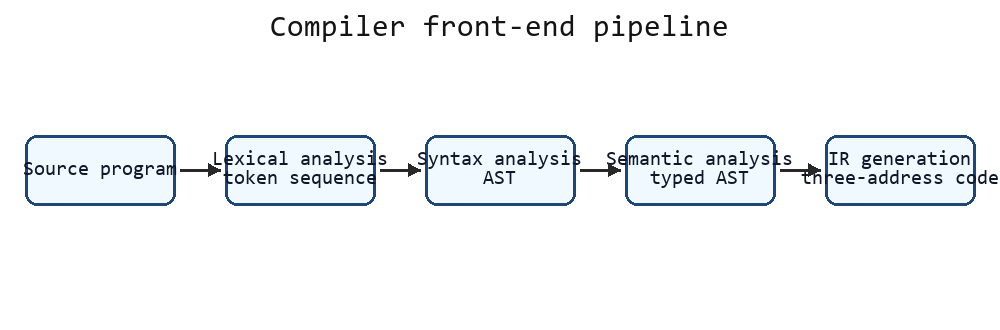
\includegraphics[width=0.82\linewidth]{figures/compiler-pipeline-11.png}
\par{\small 编译前端流水线}
\end{figure}

\begin{longtable}{|p{0.31\linewidth}|p{0.31\linewidth}|p{0.31\linewidth}|}
\hline
顺序 & 中间结果 & 编译阶段 \\
\hline
\endfirsthead
顺序 & 中间结果 & 编译阶段 \\
\hline
\endhead
① & token 序列 & 词法分析 \\
\hline
② & AST & 语法分析 \\
\hline
③ & 带类型 AST & 语义分析 \\
\hline
④ & 三地址码 & 中间代码生成 \\
\hline
⑤ & 目标代码 & 目标代码生成 \\
\hline
\end{longtable}

完整顺序：

\begin{Verbatim}[fontsize=\small,breaklines=true]
源程序 -> ① -> ② -> ③ -> ④ -> ⑤
\end{Verbatim}

\paragraph*{2. 前端、中端、后端}

\begin{longtable}{|p{0.31\linewidth}|p{0.31\linewidth}|p{0.31\linewidth}|}
\hline
部分 & 包含阶段 & 主要任务 \\
\hline
\endfirsthead
部分 & 包含阶段 & 主要任务 \\
\hline
\endhead
前端 & 词法分析、语法分析、语义分析、中间代码生成 & 理解源程序并生成 IR \\
\hline
中端 & 机器无关优化 & 在 IR 上做常量折叠、数据流优化、SSA 优化 \\
\hline
后端 & 指令选择、寄存器分配、指令调度、目标代码生成 & 把 IR 映射到目标机器 \\
\hline
\end{longtable}

\paragraph*{3. AST 与三地址码的结构差异}

\begin{longtable}{|p{0.31\linewidth}|p{0.31\linewidth}|p{0.31\linewidth}|}
\hline
对比项 & AST & 三地址码 \\
\hline
\endfirsthead
对比项 & AST & 三地址码 \\
\hline
\endhead
结构 & 树形 & 线性指令序列 \\
\hline
表达重点 & 源语言层次结构和优先级 & 显式运算步骤和临时变量 \\
\hline
例子 & \texttt{Add(2, Mul(3,4))} & \texttt{t1=3*4; t2=2+t1; x=t2} \\
\hline
适合任务 & 语义分析、类型检查 & 控制流、数据流、代码生成 \\
\hline
\end{longtable}

\paragraph*{4. 引入 IR 的两个好处}

\begin{Verbatim}[fontsize=\small,breaklines=true]
1. 解耦源语言和目标机器：多个前端可以生成同一种 IR，多个后端可以复用同一种 IR。
2. 提供统一优化载体：优化器只需处理 IR，不必分别处理不同源语言语法。
\end{Verbatim}

\paragraph*{5. phase 与 pass}

\begin{longtable}{|p{0.31\linewidth}|p{0.31\linewidth}|p{0.31\linewidth}|}
\hline
概念 & 含义 & 例子 \\
\hline
\endfirsthead
概念 & 含义 & 例子 \\
\hline
\endhead
phase & 逻辑功能阶段 & 词法分析、语义分析、寄存器分配 \\
\hline
pass & 对程序表示的一次遍历或处理 & 一次常量传播遍历、一次死代码删除遍历 \\
\hline
\end{longtable}

一个 phase 可以由多个 pass 实现；一个 pass 也可以合并几个小的处理任务。

\subsubsection*{二、DFA 最小化与等价性答案}

\paragraph*{1. DFA 五元组}

\begin{Verbatim}[fontsize=\small,breaklines=true]
Q={A,B,C,D,E}
Sigma={0,1}
q0=A
F={D,E}
delta 由题目转移表给出
\end{Verbatim}

\paragraph*{2. 划分细化}

初始按终态和非终态分组：

\begin{Verbatim}[fontsize=\small,breaklines=true]
P0 = { {D,E}, {A,B,C} }
\end{Verbatim}

细化 \texttt{\textbackslash{}\{A,B,C\textbackslash{}\}}：

\begin{longtable}{|p{0.23\linewidth}|p{0.23\linewidth}|p{0.23\linewidth}|p{0.23\linewidth}|}
\hline
状态 & 输入 0 到 & 输入 1 到 & 分组特征 \\
\hline
\endfirsthead
状态 & 输入 0 到 & 输入 1 到 & 分组特征 \\
\hline
\endhead
A & B，非终态组 & C，非终态组 & 非终态，非终态 \\
\hline
B & B，非终态组 & D，终态组 & 非终态，终态 \\
\hline
C & B，非终态组 & C，非终态组 & 非终态，非终态 \\
\hline
\end{longtable}

因此 \texttt{\textbackslash{}\{A,B,C\textbackslash{}\}} 分裂为：

\begin{Verbatim}[fontsize=\small,breaklines=true]
{A,C}, {B}
\end{Verbatim}

细化 \texttt{\textbackslash{}\{D,E\textbackslash{}\}}：

\begin{longtable}{|p{0.23\linewidth}|p{0.23\linewidth}|p{0.23\linewidth}|p{0.23\linewidth}|}
\hline
状态 & 输入 0 到 & 输入 1 到 & 分组特征 \\
\hline
\endfirsthead
状态 & 输入 0 到 & 输入 1 到 & 分组特征 \\
\hline
\endhead
D & B，即 \texttt{\textbackslash{}\{B\textbackslash{}\}} & E，即 \texttt{\textbackslash{}\{D,E\textbackslash{}\}} & \texttt{\textbackslash{}\{B\textbackslash{}\}}, \texttt{\textbackslash{}\{D,E\textbackslash{}\}} \\
\hline
E & B，即 \texttt{\textbackslash{}\{B\textbackslash{}\}} & E，即 \texttt{\textbackslash{}\{D,E\textbackslash{}\}} & \texttt{\textbackslash{}\{B\textbackslash{}\}}, \texttt{\textbackslash{}\{D,E\textbackslash{}\}} \\
\hline
\end{longtable}

二者不再分裂。最终划分：

\begin{Verbatim}[fontsize=\small,breaklines=true]
P = { {A,C}, {B}, {D,E} }
\end{Verbatim}

\paragraph*{3. 最小 DFA}

令：

\begin{Verbatim}[fontsize=\small,breaklines=true]
X={A,C}, Y={B}, Z={D,E}
\end{Verbatim}

\begin{figure}[H]\centering
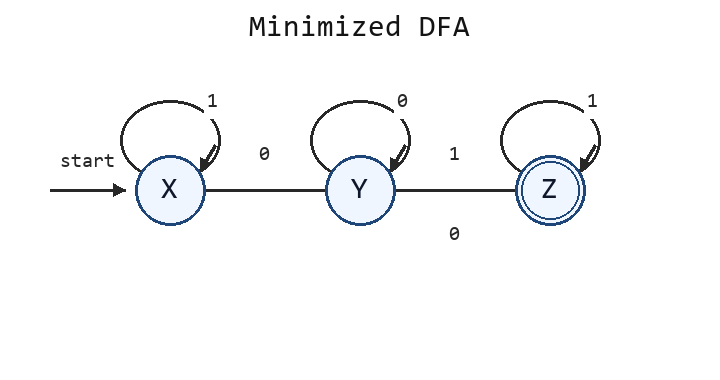
\includegraphics[width=0.82\linewidth]{figures/dfa-min-11.png}
\par{\small 最小 DFA}
\end{figure}

\begin{longtable}{|p{0.23\linewidth}|p{0.23\linewidth}|p{0.23\linewidth}|p{0.23\linewidth}|}
\hline
状态 & 输入 0 & 输入 1 & 是否终态 \\
\hline
\endfirsthead
状态 & 输入 0 & 输入 1 & 是否终态 \\
\hline
\endhead
X & Y & X & 否 \\
\hline
Y & Y & Z & 否 \\
\hline
Z & Y & Z & 是 \\
\hline
\end{longtable}

初态是 \texttt{X}，终态是 \texttt{Z}。

\paragraph*{4. 接受串和拒绝串}

\begin{longtable}{|p{0.31\linewidth}|p{0.31\linewidth}|p{0.31\linewidth}|}
\hline
类型 & 串 & 检查 \\
\hline
\endfirsthead
类型 & 串 & 检查 \\
\hline
\endhead
接受 & \texttt{01} & A -0-> B -1-> D \\
\hline
接受 & \texttt{001} & A -0-> B -0-> B -1-> D \\
\hline
接受 & \texttt{101} & A -1-> C -0-> B -1-> D \\
\hline
拒绝 & \texttt{epsilon} & 停在 A，非终态 \\
\hline
拒绝 & \texttt{0} & A -0-> B，非终态 \\
\hline
拒绝 & \texttt{11} & A -1-> C -1-> C，非终态 \\
\hline
\end{longtable}

\paragraph*{5. 乘积自动机判等价}

\begin{Verbatim}[fontsize=\small,breaklines=true]
从两个初态组成的状态对开始遍历乘积自动机。
如果能到达某个状态对 (p,q)，其中恰好一个属于接受状态，则存在区分串，两个 DFA 不等价。
如果所有可达状态对的接受性都一致，则两个 DFA 等价。
\end{Verbatim}

\subsubsection*{三、CFG、推导与 PDA 答案}

\paragraph*{1. 最左推导}

\begin{Verbatim}[fontsize=\small,breaklines=true]
S
=> a S b
=> a a S b b
=> a a epsilon b b
=> aabb
\end{Verbatim}

\paragraph*{2. 最右推导}

该文法每个中间句型中只有一个非终结符 \texttt{S}，所以最右推导与最左推导形式相同：

\begin{Verbatim}[fontsize=\small,breaklines=true]
S
=> a S b
=> a a S b b
=> a a epsilon b b
=> aabb
\end{Verbatim}

\paragraph*{3. 语言集合}

\begin{Verbatim}[fontsize=\small,breaklines=true]
L={a^n b^n | n>=0}
\end{Verbatim}

\paragraph*{4. PDA 设计}

\begin{figure}[H]\centering
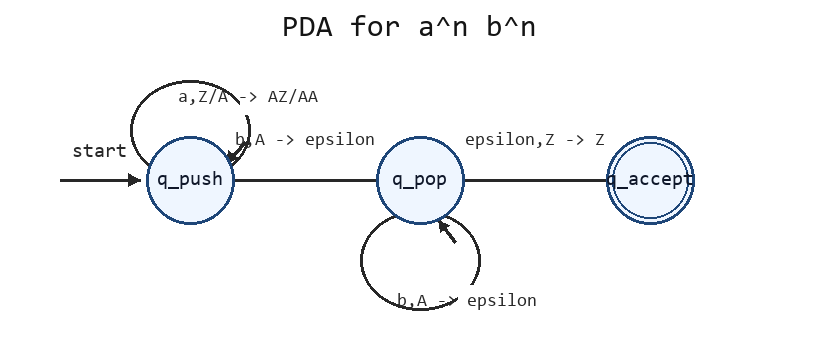
\includegraphics[width=0.82\linewidth]{figures/pda-anbn.png}
\par{\small PDA for a\textasciicircum{}n b\textasciicircum{}n}
\end{figure}


\begin{Verbatim}[fontsize=\small,breaklines=true]
状态：q_push, q_pop, q_accept
输入字母表：{a,b}
栈字母表：{Z,A}，Z 为栈底符号

delta(q_push,a,Z)=(q_push,AZ)
delta(q_push,a,A)=(q_push,AA)
delta(q_push,b,A)=(q_pop,epsilon)
delta(q_pop,b,A)=(q_pop,epsilon)
delta(q_push,epsilon,Z)=(q_accept,Z)       ; 接受空串
delta(q_pop,epsilon,Z)=(q_accept,Z)        ; 输入耗尽后接受
\end{Verbatim}

\paragraph*{5. `aabb` 的配置变化}

格式为 \texttt{(状态, 剩余输入, 栈)}，栈顶写在左侧：

\begin{Verbatim}[fontsize=\small,breaklines=true]
(q_push,aabb,Z)
|- (q_push,abb,AZ)
|- (q_push,bb,AAZ)
|- (q_pop,b,AZ)
|- (q_pop,epsilon,Z)
|- (q_accept,epsilon,Z)
\end{Verbatim}

\subsubsection*{四、二义性与 CFL 性质答案}

\paragraph*{1. 两种最左推导}

第一种最左推导，对应结构 \texttt{(id+id)*id}：

\begin{Verbatim}[fontsize=\small,breaklines=true]
E
=> E * E
=> E + E * E
=> id + E * E
=> id + id * E
=> id + id * id
\end{Verbatim}

第二种最左推导，对应结构 \texttt{id+(id*id)}：

\begin{Verbatim}[fontsize=\small,breaklines=true]
E
=> E + E
=> id + E
=> id + E * E
=> id + id * E
=> id + id * id
\end{Verbatim}

同一个输入串有两种不同语法结构，所以原文法二义。

\paragraph*{2. 改写文法}

\begin{Verbatim}[fontsize=\small,breaklines=true]
E -> E + T | T
T -> T * F | F
F -> id
\end{Verbatim}

\paragraph*{3. 为什么消除本题二义性}

\begin{longtable}{|p{0.31\linewidth}|p{0.31\linewidth}|p{0.31\linewidth}|}
\hline
层级 & 负责运算 & 作用 \\
\hline
\endfirsthead
层级 & 负责运算 & 作用 \\
\hline
\endhead
F & \texttt{id} & 基本项 \\
\hline
T & \texttt{*} & 乘法层 \\
\hline
E & \texttt{+} & 加法层 \\
\hline
\end{longtable}

\texttt{T} 出现在 \texttt{E} 中，因此乘法比加法结合得更紧；\texttt{E -> E + T} 和 \texttt{T -> T * F} 是左递归，表示相同运算符左结合。

\paragraph*{4. 正则语言与 CFL}

所有正则语言都是 CFL。理由是：正则语言能由有限自动机识别，而 PDA 可以模拟有限自动机且不使用栈。

\paragraph*{5. CFL 封闭性}

\begin{longtable}{|p{0.47\linewidth}|p{0.47\linewidth}|}
\hline
运算 & CFL 是否封闭 \\
\hline
\endfirsthead
运算 & CFL 是否封闭 \\
\hline
\endhead
并 & 是 \\
\hline
连接 & 是 \\
\hline
Kleene 星 & 是 \\
\hline
一般交 & 否 \\
\hline
补 & 否 \\
\hline
\end{longtable}

补充：CFL 对“与正则语言求交”封闭，但对两个一般 CFL 求交不封闭。

\subsubsection*{五、LL(1) 预测分析答案}

\paragraph*{1. FIRST/FOLLOW}

\begin{Verbatim}[fontsize=\small,breaklines=true]
FIRST(S)={a,b}
FIRST(A)={c,d}
FOLLOW(S)={$}
FOLLOW(A)={$}
\end{Verbatim}

\paragraph*{2. 预测分析表}

空白项写作 \texttt{error}：

\begin{longtable}{|p{0.16\linewidth}|p{0.16\linewidth}|p{0.16\linewidth}|p{0.16\linewidth}|p{0.16\linewidth}|p{0.16\linewidth}|}
\hline
非终结符 & a & b & c & d & \$ \\
\hline
\endfirsthead
非终结符 & a & b & c & d & \$ \\
\hline
\endhead
S & \texttt{S -> a A} & \texttt{S -> b} & error & error & error \\
\hline
A & error & error & \texttt{A -> c A} & \texttt{A -> d} & error \\
\hline
\end{longtable}

\paragraph*{3. LL(1) 判断}

每个表项最多一条产生式，所以文法是 LL(1)。

\paragraph*{4. 分析 `a c d \$`}

栈顶写在右侧：

\begin{longtable}{|p{0.31\linewidth}|p{0.31\linewidth}|p{0.31\linewidth}|}
\hline
分析栈 & 剩余输入 & 动作 \\
\hline
\endfirsthead
分析栈 & 剩余输入 & 动作 \\
\hline
\endhead
\texttt{\textbackslash{}\$ S} & \texttt{a c d \textbackslash{}\$} & 查 \texttt{M[S,a]}，用 \texttt{S -> a A} \\
\hline
\texttt{\textbackslash{}\$ A a} & \texttt{a c d \textbackslash{}\$} & 匹配 \texttt{a} \\
\hline
\texttt{\textbackslash{}\$ A} & \texttt{c d \textbackslash{}\$} & 查 \texttt{M[A,c]}，用 \texttt{A -> c A} \\
\hline
\texttt{\textbackslash{}\$ A c} & \texttt{c d \textbackslash{}\$} & 匹配 \texttt{c} \\
\hline
\texttt{\textbackslash{}\$ A} & \texttt{d \textbackslash{}\$} & 查 \texttt{M[A,d]}，用 \texttt{A -> d} \\
\hline
\texttt{\textbackslash{}\$ d} & \texttt{d \textbackslash{}\$} & 匹配 \texttt{d} \\
\hline
\texttt{\textbackslash{}\$} & \texttt{\textbackslash{}\$} & 接受 \\
\hline
\end{longtable}

\paragraph*{5. 输入 `a c c \$` 的错误表项}

分析过程会匹配 \texttt{a}，然后两次使用 \texttt{A -> c A} 匹配两个 \texttt{c}。此时栈顶仍为 \texttt{A}，当前输入为 \texttt{\textbackslash{}\$}，查表：

\begin{Verbatim}[fontsize=\small,breaklines=true]
M[A,$] = error
\end{Verbatim}

因此具体错误表项是 \texttt{M[A,\textbackslash{}\$]}。
\end{document}
